\documentclass[a4paper, 11pt]{report}
\usepackage[utf8]{inputenc}
\usepackage[T1]{fontenc}
\usepackage[colorlinks=true, urlcolor=purple, linkcolor=blue, pdftitle={Projet Optimisation}, pdfauthor={Adrien TALATIZI, Alexandre MARIN}, pdfsubject={optimisation}, pdfkeywords={master I.M.P.E., optimisation, MATLAB}]{hyperref}
\usepackage[french]{babel}
\usepackage{xspace}
\usepackage{textcomp}
\usepackage[table]{xcolor}

\usepackage{array}
\usepackage{amsmath}
\usepackage{amssymb}
%\usepackage{amsthm}
%\usepackage[french]{algorithm2e}
\usepackage{graphicx}
\usepackage{listings}
\usepackage{mathrsfs}
\usepackage[hmargin=2.0cm, bottom=2cm]{geometry}

\newcounter{question}
\renewcommand\thesection{\arabic{section}}
\renewcommand\thequestion{Question 1.4.\arabic{question}}
\newcommand\question{\addtocounter{question}{1}\vspace*{1cm}{\raggedright\textbf{\thequestion}}\par\vspace*{0.5cm}}


%important quantities
\newcommand\propellantsvlct[1]{\mathrm{v}_{\mathrm{e}\,#1}}%velocity of the propellants
\newcommand\masspropel[1]{\mathrm{m}_{\mathrm{e}\,#1}}%propelling velocity
\newcommand\massstruct[1]{\mathrm{m}_{\mathrm{s}\,#1}}%mass of the structure
\newcommand\constructidx[1]{\mathrm{k}_{#1}}%constructive index
\newcommand\initmass[1]{\mathrm{M}_{\mathrm{i}\,#1}}%initial mass
\newcommand\finalmass[1]{\mathrm{M}_{\mathrm{f}\,#1}}%final mass
\newcommand\propellingvlct{\mathrm{V}_{\mathrm{p}}}%propelling velocity
\newcommand\realvlct{\mathrm{V}_{\mathrm{r}}}%real velocity
\newcommand\targetvlct{\mathrm{V}_{\mathrm{c}}}%target velocity
\newcommand\payload{\mathrm{m}_{\mathrm{u}}}%payload
\newcommand\targetalt{\mathrm{H}_{\mathrm{c}}}%target altitude
\newcommand\durcombustion[1]{t_{\mathrm{c}\,#1}}%duration of combustion

\includeonly{intro, descSQP, test_cases, global, analytical_part, results}


\begin{document}

\lstset{%
basicstyle=\color{black}\ttfamily,%
keywordstyle=\color{blue}\bfseries\ttfamily,%
identifierstyle=, %
commentstyle=\color{green}\slshape, %
stringstyle=\ttfamily, %
showstringspaces=true,%
language=MATLAB,%
frame=none,%
numbers=none}



\begin{titlepage}
\author{Adrien TALATIZI\\ Alexandre MARIN}
\date{pour le 7 janvier 2020}
\title{Projet Optimisation\\ Optimisation d'un lanceur spatial}
\maketitle
\end{titlepage}

\tableofcontents


\section{Introduction}

Ce projet d'optimisation, qui est un module du master \emph{Ingénierie Mathématique Pour l'Entreprise}, consiste à configurer un lanceur spatial afin de mettre sur orbite un satellite. Dans notre cas, il s'agit d'amener une masse utile $m_{\textrm{u}}=1~500~\textrm{kg}$ en orbite, à l'altitude $R_{\textrm{c}}=200~\textrm{km}$.

Dans ce rapport, nous décrivons d'abord succinctement la fonction \lstinline+SQP+, nous résumons les cas tests, nous expliquons ensuite l'optimisation du lanceur et nous présentons enfin les résultats issus de cette optimisation.

Les réponses aux questions en rapport avec la résolution analytique sont également données.

\vspace{2cm}

L'arborescence du projet s'organise comme suit, avec ces dossiers :
\vspace{1cm}
\begin{itemize}
\item\lstinline+SQP+ contient les fichiers nécessaires au fonctionnement de l'algorithme SQP ;
\item\lstinline+simulator+ contient deux fonctions permettant l'intégration numérique pour le problème de trajectoire ;
\item\lstinline+solving+ contient des scripts résolvant les problèmes posés dans le cadre de ce projet ;
\item\lstinline+tests+ rassemble des tests des fonctions contenues dans les dossiers \lstinline+SQP+ et \lstinline+simulator+.
\end{itemize}

%Adrien's part
\section{Description de méthode SQP}\bigbreak


L'objectif de la méthode SQP est de résoudre les condictions KKT : $\nabla$L$(x,\lambda)$=0.\\
Pour cela, nous nous basons sur la méthode de Newton. \`A chaque itération, la résolution du système linéaire\\


\begin{equation*}
\begin{cases}
\nabla_{xx}^2 $L$(x_k,\lambda_k)d_k + \nabla c(x_k)d_{\lambda}=-\nabla_x $L$(x_k,\lambda_k)\\
\nabla c(x_k)^{T} d_x = -c(x_k)
\end{cases}
\end{equation*}

Revient à résoudre un problème de minimisation quadratique \\
\begin{equation*}
\begin{cases}
\displaystyle \min_{d_{QP} \in {R^n}} \frac{1}{2}d_{QP}^{T}\nabla_{xx}^2$L$(x_k,\lambda_k) d_{QP} + 
\nabla_x $L$(x_k,\lambda_k)^{T}d_{QP} \\ $sous   $  \nabla c(x_k)^{T}d_{QP}+c(x_k) = 0
\end{cases}
\end{equation*}

\par 
Un théorème du cours nous assure existence et unicité de la solution d'un tel problème si Q := $\nabla_{xx}^2 $L$(x_k,\lambda_k)$ est définie positive.
L'évaluation de la solution exacte - si elle existe - est très coûteuse. En effet, il faut calculer un Hessien ainsi que plusieurs inverses et plusieurs produits matriciels. \\
\par 
L'idée au long de cette méthode SQP est d'approximer toutes les quantités coûteuses en calcul et de s'assurer de l'amélioration de la solution à chaque étape par des moyens astucieux.\medbreak
Ainsi,\\
\renewcommand{\labelitemi}{\textbullet}
\begin{itemize}
\item On calcule une approximation H du Hessien au lieu de calculer Q : \\
- Nous choisissons d'utiliser la forume BFGS pour calculer cette approximation H car elle présente l'avantage de fournir 
une matrice définie positive qui ne nécéssite pas de modification.\\
\item On utilise la méthode de globalisation pour s'assurer que le déplacement calculé est une amélioration :\\
\indent- Pour s'assurer que $\|    \nabla $L$(x_{k+1},\lambda_{k+1})   \| < \|    \nabla $L$(x_{k},\lambda_{k})   \|$,
on effectue un test sur la fonction "mérite" F(x) car $\nabla $L est coûteux à calculer. \\
\indent- Si la solution QP n'est pas acceptable, on la garde comme direction de recherche et on cherche un pas "s" vérifiant la condiction d'Armijo.\\
\end{itemize}
\par

Cependant, l'algorithme SQP présente les mêmes défauts que l'algorihme de Newton et ne converge donc pas vers une direction unique. Pour éviter d'atteindre des solutions non-physiques, on fait des projections sur des bornes relativement proches de la solution réelle. Il faut donc avoir en avance une idée de cette solution.\bigbreak
\indent Le rajout de conditions d'arrêt permet de limiter le temps de calcul. L'algorithme SQP est arrêté si :\medbreak
- Le déplacement de la solution est négligeable.\\
\indent- La différence entre $\|    \nabla$L$(x_{k+1},\lambda_{k+1})   \| $ et $\|    \nabla $L$(x_{k},\lambda_{k})   \|$ est estimée suffisamment petite.\\
\indent- On a appelé suffisamment de fois les fonctions f et c.\\
\indent- Les conditions d'arrêt de base de l'algorithme de Newton ( $\| \nabla $L$ \| < \epsilon$ et $n_{iter} < K$, $K$ posé à l'avance).\\
\par
Afin d'établir les tableaux, l'algorithme SQP renvoie :\medbreak
\indent- La solution "x" calculée,\\
\indent- Le multiplicateur de Lagrange "$\lambda$",\\
\indent- Le nombre d'itérations de l'algorithme "k",\\
\indent- $\| \nabla$L$ \|$
\indent- Les valeurs de f et c atteintes en x, f(x) et c(x).\\
\indent- La valeur finale de $\rho$ et le nombre d'appels de f et c.
\bigbreak
\textit{Note : Comme conseillé dans le PDF, SQP prend en argument "problem" qui est soit un pointeur vers une fonction, soit un domaine de deux cellules contenant le pointeur vers la fonction et les indices des contraintes sélectionnées. Cependant, pour le reste du programme, nous n'utliserons que le premier type d'argument, à savoir une fonction qui renvoie un vecteur "fonction" et "contrainte".}

%Adrien's part
\section{Présentation des résultats sur les deux cas tests}

\begin{center} \emph{\textbf{PREMIER CAS TEST} : polynôme}\\\end{center}

\renewcommand{\labelitemi}{\textbullet}
\begin{itemize}
\item On définit la fonction test \textit{f} t.q.\\
$f(x_1,x_2,x_3,x_4,x_5) = (x_1-1)^2+(x_1-x_2)^2 + (x_2 - x_3)^3 + (x_3 - x_4)^4 + (x_4 - x_5)^4$\\
\item Et la contrainte \textit{c} t.q.\\
$c(x_1,x_2,x_3,x_4,x_5) =
(x_1 + x_2)^2 + x_3^2 - 3\sqrt{2} - 2 , 
x_2 - x_3^2 + x_4 - 2\sqrt{2} + 2 , 
x_{1}x_{5} - 2)^{T}$;\bigbreak
\end{itemize}

\begin{itemize}
\item On prend comme point de départ de l'algorithme SQP : $x^0 = (-1 ; 2 ; 1 ; -2 ; -2)^{T}$\\
\indent avec pour objectifs : $x^{*} = (-1.2366 ; 2.4616 ; 1.1911 ; -0.2144 ; -1.6165)^{T}$ et $f(x^{*}) = 28.4974$\\
\end{itemize}
Les résultats sont stockés dans le tableau suivant : \smallbreak
{\renewcommand{\arraystretch}{1.5}\setlength{\tabcolsep}{3pt}
\begin{table}[h]\centering \small\begin{tabular}{|c|c|c|c|c|c|c|}
	\hline
 	iter & x & f(x) & $\| $c(x)$ \|$ & $\|    \nabla $L$  \|$ & rho & appels de f et c\\
	\hline
 	0 & $( -1, 2, 1, -2, -2 )^{T}$ & 95.0 & 2.8935 & 62.7595 & / & 6\\
	\hline
 	1 & $(-0.937, 2.16, 1.49, 0.0856, -1.9165)^{T}$ & 33.62 & 0.877 & 194.896 & 52.196759 & 12\\
	\hline
 	2 & $( -1.54, 2.2954, 1.49, 0.09, -1.32 )^{T}$ & 29.4057 & 0.73 & 42.71 & 12.824709 & 20\\
	\hline
 	3 & $( -0.9, 2.49, 1.07, -0.51, -1.85 )^{T}$ & 27.871 & 0.32 & 6.514 & 10.790444 & 26\\
	\hline
 	4 & $( -1.21, 2.45, 1.21, -0.17, -1.592 )^{T}$ & 27.94 & 0.078 & 2.52 & 10.112978 & 32\\
	\hline
 	5 & $( -1.2595, 2.4669, 1.19, -0.22, -1.588 )^{T}$ & 28.53 & 98e-5 & 1.454 & 10.005331 & 38\\
	\hline
 	6 & $( -1.2393, 2.4623, 1.19, -0.22, -1.61)^{T}$ & 28.504 & 518e-6 & 0.237 & 9.942327 & 44\\
	\hline
 	7 & $( -1.237, 2.46, 1.19, -0.216, -1.6169 )^{T}$ & 28.50865 & 8.178e-06 & 9.963e-3 & 9.897096 & 50\\
	\hline
 	8 & $( -1.237, 2.46, 1.19, -0.21565, -1.6168 )^{T}$ & 28.508725 & 2.61e-09 & 48e-6 & 9.896991 & 56\\
	\hline
 	9 & $( -1.237, 2.462, 1.19, -0.21565, -1.6168 )^{T}$ & 28.5087 & 2.077e-12 & 3.1395e-07 & 9.896981 & 62\\

	\hline
\end{tabular}\end{table}
}\normalsize
\bigbreak
\textit{Note : les résultats obtenus sont bien conformes aux résultats attendus. On remarquera que sans les bornes, SQP converge vers d'autres minima locaux. Il est donc important de choisir ces bornes proches de la solution attendue. On choisit donc un intervalle de 0.6
autour de celle-ci.}
\newpage





\begin{center}\emph{\textbf{SECOND CAS TEST} : masses d'ergols de la fusée Ariane 1}\\\end{center}





\begin{itemize}
\item On définit la fonction test \textit{f} t.q.\\
$f(x_1,x_2,x_3) = 1700+1.1101x_1 + 1.1532x_2 + 1.2154x_3$\\
\item Et la contrainte \textit{c} t.q.\\
$c(x_1,x_2,x_3) =$\\
\smallbreak
$4344.3ln(\frac{1700+1.2154x_3}{1700+0.2154x_3}) 
+ 2922.4ln(\frac{1700+1.2154x_3+1.1532x_2}{1700+0.2154x_3+0.1532x_2}) 
+ 2647.2ln(\frac{1700+1.2154x_3+1.1532x_2+1.1101x_1}{1700+0.2154x_3+0.1532x_2+0.1101x_1}) 
-11527$

\bigbreak

\item On prend comme point de départ de l'algorithme SQP : $x^0 = (115000, 35000, 6000)^{T}$ qui est la moyenne des bornes\\
\indent avec pour objectifs : $x^{*} = (145349 ; 31215 ; 7933)^{T}$ et $f(x^{*}) = 208691$\\
\end{itemize}
Les résultats sont stockés dans le tableau suivant : \smallbreak
{\renewcommand{\arraystretch}{1.5}
\begin{table}[h]\centering \small\begin{tabular}{|c|c|c|c|c|c|c|}
	\hline
 	iter & x & f(x) & $\| $c(x)$ \|$ & $\|    \nabla $L$  \|$ & rho & appels de f et c\\
	\hline
	0 & $(115000, 35000, 6000)^{T}$ & 177015.90 & 361.36 & 361.36 & / & 4\\
	\hline
	1 & $(115970.49, 35416.328, 10000)^{T}$ & 183434.95 & 273.45 & 1564.81 & 81642.55 & 8\\
	\hline
	2 & $(127626.0, 44731.2, 5870.50)^{T}$ & 202096.70 & 199.55 & 87809.94 & 1001129.48 & 12\\
	\hline
	3 & $(137284.567, 50000, 6870.88 )^{T}$ & 220110.46 & 21.18 & 7113.2 & 119425.29 & 16\\
	\hline
	4 & $(138609.19, 50000, 6991.44 )^{T}$ & 221727.45 & 1.35& 185.21 & 3332.76 & 20\\
	\hline
	5 & $(138700.45, 49991.19216, 6999.994 )^{T}$ & 221829.01 & 13e-4 & 3.84 & 90.44 & 24\\
	\hline
	6 & $(138700.47, 49971.01733, 7000.62 )^{T}$ & 221806.52 & 6.4e-05 & 3.13 & 76.58 & 28\\
	\hline
	7 & $(138539.77, 20000, 8529.26 )^{T}$ & 188923.47 & 235.69 &235.71 & 128.95 & 32\\
	\hline
	8 & $(137507.1, 30996.5, 7875.68)^{T}$ & 199663.91 &  79.98 & 79.98 & 100.46 & 36\\
	\hline
	9 & $(143378.6, 32532.79, 8406.05 )^{T}$ & 208598.11 & 3.37 & 3.44 & 126.30 & 40\\
	\hline
	10 & $(143403.19, 32874.4, 8379.81 )^{T}$ & 208987.45 & 0.045 & 0.61 & 122.72 & 44\\
	\hline
\end{tabular}
\end{table}}
\bigbreak
\textit{Note : les résultats obtenus sont bien conformes au résultats attendus. On remarquera que sans les bornes, SQP converge vers d'autres minima locaux. Il est donc important de choisir ces bornes proches de la solution attendue. On choisit donc de poser la borne supérieure comme étant $(170000 , 50000 , 10000)^{T}$ et la borne inférieure comme $(60000 , 20000 , 2000)^{T}$. Cela nous évite de plus de converger vers des solutions non physiques.}


%Adrien's part
\section{Optimisation \textbf{lanceur}}
%Organisation :\medbreak
%\subsection{Approche générale}
%\subsection{Stratégies sur le SQP}
%\subsubsection{Choix sur BFGS}
%\subsubsection{Choix sur les projections}
%\subsection{Partie analytique}
%\subsubsection{Idée pré-résolution}
%\subsubsection{Construction}
%\subsection{\'Ecriture des problèmes}
%\subsubsection{Problème d'étagement}
%\subsubsection{Problème de trajectoire}
%\subsection{Résolution des problèmes via SQP}
%\indent a) Résolution du problème d'étagement\\
%\indent b) Résolution du problème de trajectoire\\
%\subsection{Problème final}
%\bigbreak


\subsection{Approche générale}\medbreak

Nous procédons par étapes afin de réaliser le lanceur. La première est la réalisation de l'algorithme SQP. Afin de faciliter son fonctionnement, il faut avoir une idée de la solution vers laquelle il doit converger. On utilise donc la partie analytique à l'aide de l'algorithme de Newton pour approcher les masses d'ergols solutions de notre problème. C'est le programme \texttt{"analytical\_approach"}.\\
On définit la fonction problème d'étagement (resp. problème de trajectoire) dans \texttt{"stageproblem"} (resp. \texttt{"pathproblem"}). Afin de trouver la solution du problème d'étagement, on définit le script \texttt{"solve\_stageproblem"} qui applique SQP au probème d'étagement. Pour la solution du problème de trajectoire, on utilise \texttt{"solve\_pathproblem"} qui fait plusieurs applications astucieuses de SQP sur les 4 angles.\\
Enfin, pour les itérations sur la vitesse propulsive, on définit un programme \texttt{"set\_config"} dans lequel on fera plusieurs applications inspirées de \texttt{"solve\_pathproblem"} et \texttt{"solve\_stageproblem"} à l'aide des fonctions \texttt{"path\_solver"} et \texttt{"stage\_solver"}.\bigbreak


\subsection{Partie analytique}\medbreak

\subsubsection{Idée pré-résolution}\medbreak
L'idée de pré-résoudre le problème a été évoquée plusieurs fois. La partie analytique que l'on trouve dans le programme \texttt{"analytical\_approach"} a cette vocation. On utilise l'exercice du sujet pour résoudre le problème équivalent au problème d'étagement (1 équation à 1 inconnue) à l'aide de l'algorithme de Newton. Une fois $x_3$ trouvé, on en déduit $x_1$ et $x_2$ et on remonte aux 3 masses d'ergols.\\
La variable KKT sert à vérifier que la condition KKT d'ordre 1 est respectée. KKT = 0 ici, c'est donc bien le cas.\medbreak
\subsubsection{Construction}\medbreak
Comme le reste de nos algorithmes, ce script travaille sur des variables globales initialisées par la fonction de type void \texttt{"data()"}. Ce choix de travailler sur les variables globales permet de traiter les problèmes de trajectoire et d'étagement sans modifier leurs arguments : on n'a pas à copier un grand nombre de valeurs pour chaque fonction.\bigbreak



\subsection{\'Ecriture des problèmes}\medbreak
\subsubsection{Problème d'étagement}\medbreak
Le problème d'étagement est encodé dans \texttt{"stageproblem"}. La fonction prend en argument un vecteur \texttt{"m"} des masses d'ergol et retourne deux réels : \texttt{Mi} et \texttt{y}. \texttt{Mi} est la masse initiale de la fusée, construite à partir des masses d'ergol. Il s'agit de la quantité à minimiser dans le problème d'optimisation. y est la valeur de la fonction contrainte du problème d'étagement prise en \texttt{"m"} .\medbreak
\subsubsection{Problème de trajectoire}\medbreak

Afin de coder le problème de trajectoire, on doit résoudre une EDO. La fonction \texttt{"pathproblem"} prend en argument un vecteur \texttt{"theta"} de quatre composantes et renvoie "-" la norme de la vitesse (réécriture du problème avec l'idée max = "-" min) et la valeur la contrainte normalisée selon les $\theta_0, \theta_1, \theta_2, \theta_3$ dans \texttt{"theta"}. \\
La principale difficulté est de résoudre l'EDO. Pour cela, on construit la fonction "rocketpath" qui se servira elle-même de \texttt{"odefunc"}.\\
\texttt{"rocketpath"} renvoie 6 vecteurs : tous les $R_x$ et $R_y$ stockés dans \texttt{R}, tous les $V_x$ et $V_y$ stockés dans \texttt{V}, toutes les masses stockées dans \texttt{M} et l'ensemble des temps d'intégration \texttt{"tspanout"} (à chaque temps correspond une donnée ($R_x,R_y,V_x,V_y$, M). Les arguments donnés sont les 4 thetas. On commence par initialiser \texttt{"R", "V", "tspan"} qui servira de bornes d'intégration pour ODE45 et \texttt{"tspanout"} qu'on remplira avec les temps ressortis par ODE45. On boucle sur les 3 changements d'angle avec ODE45 qui prend en appel la fonction \texttt{"odefunc"}. Durant cette boucle, on concatène les résultats dans \texttt{"res"} et \texttt{"tspanout"}. Enfin, on extrait les résultats dans 2 doubles vecteurs \texttt{"R"} et \texttt{"V"} et un vecteur "M".\\

La fonction \texttt{"odefunc"} décrit le second membre de l'EDO. Elle prend en argument les données de l'étage en cours de consommation. On définit dedans les constantes physiques puis on remplit le vecteur dydt en fonction du vecteur y construit précédemment.\medbreak

\subsection{Résolution des problèmes via SQP}\medbreak
On dispose donc de deux fonctions problèmes d'étagement et de trajectoire. Il s'agit maintenant de résoudre ces deux problèmes.\\
On va construire deux scripts pour résoudre ces problèmes séparémment et deux fonctions reprennant les principes respectifs des scripts.\medbreak


\subsubsection{Résolution du problème d'étagement}\medbreak

On commence par créer le script \texttt{"solve\_stageproblem"} : \\
\indent - On reprend la solution analytique trouvée dans \texttt{"analytical\_approach"} qu'on pose comme \texttt{"m0"} et on pose les bornes à plus et moins 1500, 1000, 500. On va utiliser SQP donc on place les déplacements minimum ainsi que les maxima d'itérations et d'appels sur f et c. On applique SQP pour trouver les masses d'ergol qui minimisent la masse finale de la fusée. Ce vecteur de 3 masses d'ergol \texttt{"m\_e" }est stocké dans un fichier \texttt{"m\_e.mat"}.\medbreak

Nous créons ensuite \texttt{"stage\_solver"} qui est une fonction de type "void" là encore. On initialise les bornes proches de la solution analytique. L'idée est ensuite, pour un nombre d'essais donné, de générer aléatoirement un vecteur de masse d'ergol dans cet intervalle. Après application de SQP, on teste si $\|    \nabla $L$   \|$ est plus petit qu'une tolérance proche de 0. C'est une façon d'exiger une bonne vérification des conditions KKT d'ordre 1. Dans le cas où aucun vecteur ne vérifie cette condition, on s'assure que l'algorithme retourne quand même le vecteur le plus proche de vérifier cette condition grâce à un second test dans la boucle. Celui-ci remplace l'ancien vecteur des masses d'ergols par celui généré dans la boucle si $\|    \nabla $L$_{nouveau}   \| < \|    \nabla $L$_{ancien}   \|$.\medbreak


\subsubsection{Résolution du problème de trajectoire}\medbreak

On commence par créer le script \texttt{"solve\_pathproblem"} : \\
\indent - On respecte les conseils donnés dans le PDF. On commence par charger \texttt{"m\_e.mat"}. Les masses initiales \texttt{"Mi"} à chaque étage ainsi que les temps de combustion "t\_c" se déduisent des masses d'ergol et des données du problème présentes dans \texttt{"data()"}.\\
On commence par trouver 4 thetas à la main qui donnent une trajectoire assez correcte. On applique \texttt{"rocketpath"} sur ce vecteur \texttt{"theta"} := ($\theta_0,\theta_1,\theta_2,\theta_3$) pour obtenir vitesse et position au fil du temps. Le but est ensuite d'optimiser $\theta_2$, $\theta_3$ puis $\theta_1$, $\theta_2$, $\theta_3$ via SQP appliqué sur des fonctions anonymes. On applique enfin un dernier SQP sur tous les thetas pour améliorer encore la solution. On affiche dans des graphiques les trajectoires et vitesses avec l'altitude visée et la Terre pour observer l'amélioration. Afin de vérifier la cohérence des résultats, on affiche également dans 3 graphiques différents la vitesse, la masse et la distance par rapport à la Terre en fonction du temps.\medbreak

Nous créons ensuite \texttt{"path\_solver"}. Elle renvoie les thetas, la trajectoire. Comme toujours, on initialise les critères de contôle de la solution et les critères d'arrêt du SQP. Le but est d'obtenir un bon candidat pour \texttt{"theta"} avant d'optimiser $\theta_2$, $\theta_3$ puis $\theta_1$, $\theta_2$, $\theta_3$ via SQP appliqué sur des fonctions anonymes. On reprend l'idée servant à trouver un bon candidat pour les masses d'ergol en générant des thetas aléatoires dans l'intervalle et on arrête si un vecteur est proche de vérifier les conditions KKT d'ordre 1. Si un tel vecteur n'existe pas, on prend le meilleur des vecteurs générés au cours de la boucle.\medbreak

\subsection{Problème final}\medbreak

Le problème final est résolu dans le script \texttt{"set\_config"}. On utilisera \texttt{"path\_solver"} et \texttt{"stage\_solver"}.\\
On appelle \texttt{"data()"} pour initialiser les valeurs. On poursuit cette initialisation en appelant \texttt{"stage\_solver()"} afin de paramétrer les masses d'ergol et les $\texttt{(M\_i)}_j$ et $\texttt{(t\_c)}_j$ qui en découlent. On pose la tolérance à 10 m/s et le nombre d'itérations maximum à 5.\\
Dans une boucle \texttt{"while"}, on actualise la vitesse \texttt{V\_p}, on exécute successivement \texttt{"stage\_solver"} et \texttt{"path\_solver"}. L'exécution de \texttt{"stage\_solver"} est suivie d'une mise à jour des masses \texttt{M\_i} et des temps de combustion qui seront utilisés par \texttt{"path\_solver"}.\\
Cette boucle s'arrête une fois que la vitesse réelle est à moins de 10m/s de la vitesse visée ou qu'on dépasse le nombre d'itérations maximum.
\section{Résolution analytique du problème d'étagement}

On reprend les notations de l'énoncé, indications comprises.

\question Notons que pour $j\in\{1,2,3\}$,
\begin{align*}
\dfrac{\initmass{j+1}}{\initmass{j}} &= \dfrac{\finalmass{j}-\massstruct{j}}{\initmass{j}} =%
\dfrac{\finalmass{j}-\constructidx{j}\masspropel{j}}{\initmass{j}} \\ &= \dfrac{\finalmass{j}-\constructidx{j}(\initmass{j}-\finalmass{j})}{\initmass{j}} = \dfrac{1+\constructidx{j}}{x_{j}}-\constructidx{j}\text{.}
\end{align*}

Notons $\varphi$ l'application qui envoie $(\masspropel{1},\masspropel{2},\masspropel{3})$ sur $x$ par la formule
\[x_{j} = 1 + \dfrac{\masspropel{j}}{\payload + \sum_{j<l\leqslant 3}(1+\constructidx{l})\masspropel{l} \,+ \constructidx{j}\masspropel{j}}\text{.}\]
Alors $\varphi$ est bijective car pour tout $j\in\{1,2,3\}$
\[\masspropel{j}=\dfrac{\payload + \sum_{j<l\leqslant 3}(1+\constructidx{l})\masspropel{l}}{1+\constructidx{j}(1-x_{j})}\]
et donc $J=-f\circ \varphi$. La reformulation de la contrainte étant immédiate, les deux problèmes considérés sont équivalents.

\question Si $x$ est un minimiseur local de $f$ sous la contrainte $c$, comme ces deux fonctions sont de classe $\mathscr{C}^1$ et que la contrainte en $x$ est forcément qualifiée, il existe $\lambda\in\mathbb{R}$ tel que, pour tout $j\in\{1,2,3\}$
\[\dfrac{\partial f}{\partial x_{j}}(x) + \lambda\dfrac{\partial c}{\partial x_{j}}(x) = 0\]
avec
\[\dfrac{\partial f}{\partial x_{j}}(x) = y_{j+1}\,y_{j+2}\left(\dfrac{1+\constructidx{j}}{x_{j}^{2}}\right)%
,\; \dfrac{\partial c}{\partial x_{j}}(x) = \dfrac{\propellantsvlct{j}}{x_{j}}\]
en considérant des indices \emph{modulo} $3$.

En multipliant l'équation ci-desssus par $x_j$ et en remarquant que
\[f(x)=-y_{1}\,y_{2}\,y_{3},\; 1+\dfrac{\constructidx{j}}{y_{j}}=(1-\Omega_{j}x_{j})^{-1}\]
on obtient
\[\propellantsvlct{j}(1-\Omega_{j}x_{j}) = \dfrac{f(x)}{\lambda}\text{.}\]

\question Dans l'équation qui précède, le membre de droite ne dépend pas de $j$, donc
\[x_{j} = \dfrac{1}{\Omega_{j}}\left[1-\dfrac{\propellantsvlct{3}}{\propellantsvlct{j}}(1-\Omega_{3}x_{3})\right]\]
et on voit que le problème revient à résoudre $c(x)=0$ où $x_1$ et $x_2$ s'expriment en fonction de $x_3$.

\question On considère une vitesse propulsive $\propellingvlct = 1.2\,\targetvlct$. Dans le fichier \verb+analytical_approach.m+ du dossier \verb+solving+, nous résolvons cette équation en $x_3$ avec la méthode de Newton. On obtient

\begin{center}
$\begin{array}{|c|c|c|c|c|c|}\hline
x_3 & \masspropel{1} & \masspropel{2} & \masspropel{3} & \mathrm{M}_{0} & \lambda\\\hline
3,118\,9 & 26\ 981\text{ kg}& 12\ 704\text{ kg} & 5\ 516\text{ kg} & 52\ 408\text{ kg} & -1,354\,7\cdot 10^{-5}\\\hline
\end{array}$
\end{center}

La troisième équation donnée par le théorème de K.K.T. nous conduit au nombre $-3,47\cdot 10^{-18}$.


\section{Résultats}

\subsection{Résultats numériques}

Les grandeurs physiques ont pour unités celles du système international.

Les itérations sur la vitesse propulsive sont effectuées dans le script \lstinline+set_config.m+~: les problèmes d'étagement et de trajectoire sont résolus respectivement grâce aux fichiers \lstinline+stage_solver.m+ et \lstinline+path_solver.m+.

Voici les résultats issus de l'exécution de \lstinline+set_config.m+~:

\[\begin{array}{|c|c|c|c|c|c|}\hline
\text{itération} & \masspropel{} & \propellingvlct & \realvlct & \mathrm{M}_0 & \theta\\ \hline
1 & \begin{pmatrix}27\,144\\ 12\,564\\ 5\,501\end{pmatrix} & 9\,341 & 7\ 801 & 52\,408 & %
\begin{pmatrix}0,053\\ -0,013\,768\\ 0,326\,8\\ 0,138\,06\end{pmatrix}\\\hline
2 & \begin{pmatrix}26\,841\\ 12\,496\\ 5\,491\end{pmatrix} & 9\,324 & 7\ 781 & 51\,984 & %
\begin{pmatrix}0,053\\ -0,013\,727\\ 0,327\,56\\ 0,139\,06\end{pmatrix}\\\hline
\end{array}\]

La vitesse cible $\targetvlct$ vaut dans notre cas $7\,784,26$.

\subsection{Graphes : trajectoire, altitude, vitesse et masse}

Les graphes présentés ici correspondent à la configuration optimale du lanceur.

Voici les durées de combustion et instants $t_j$ de fin de combustion pour chaque étage~:

\[\begin{array}{|c|c|c|}\hline
\durcombustion{1} & \durcombustion{2} & \durcombustion{3}\\\hline
89,5 & 166,9 & 298,7\\\hline
\end{array}\]

\[\begin{array}{|c|c|c|}\hline
t_{1} & t_{2} & t_{3}\\\hline
\durcombustion{1} & 256,4 & 555,1\\\hline
\end{array}\]

\clearpage
\begin{center}
\begin{figure}[htbp]
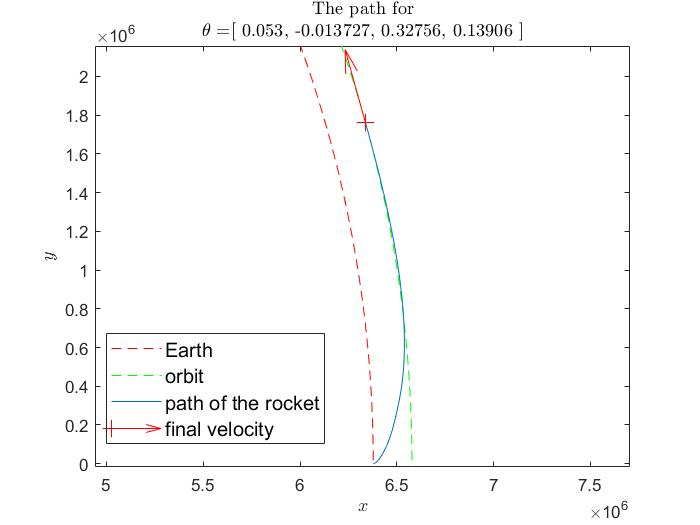
\includegraphics[scale=0.65]{./graphs/path.jpg}
\caption{trajectoire de la fusée et vecteur vitesse final}
\end{figure}
\end{center}

D'après ce graphe, il semble que l'altitude cible est atteinte et que le vecteur vitesse final est bien tangent à l'orbite visée.

\clearpage
\begin{center}
\begin{figure}[t]
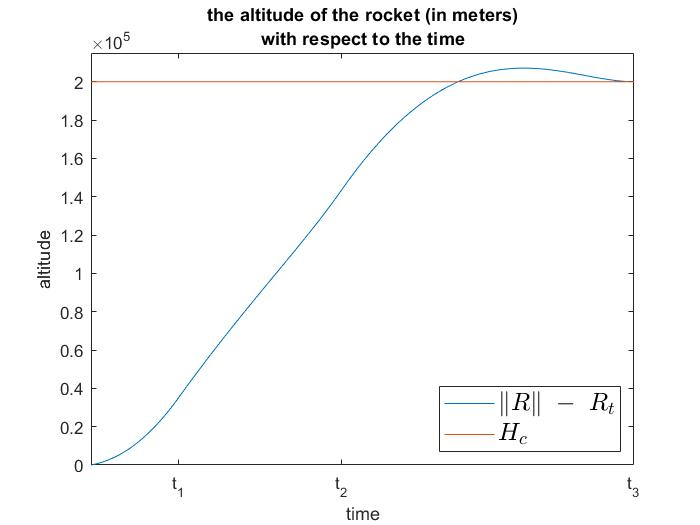
\includegraphics[scale=0.65]{./graphs/altitude.jpg}
\caption{altitude de la fusée en fonction du temps}
\end{figure}
\end{center}

L'altitude cible est bien atteinte selon ce graphe.

\clearpage
\begin{center}
\begin{figure}[t]
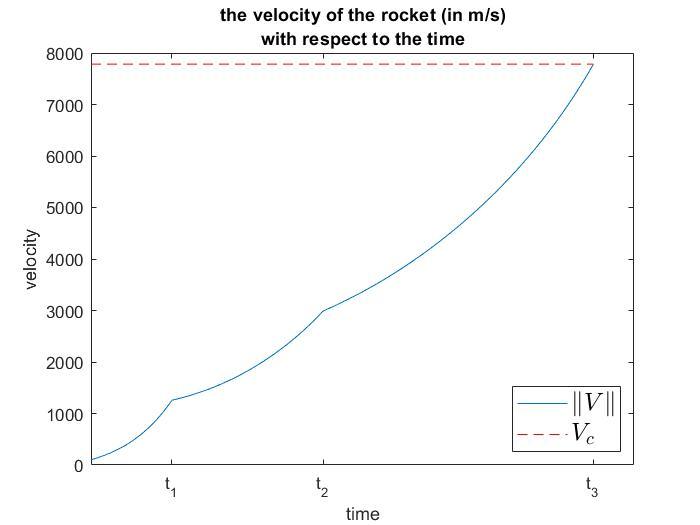
\includegraphics[scale=0.65]{./graphs/velocity.jpg}
\caption{vitesse de la fusée en fonction du temps}
\end{figure}
\end{center}

On peut s'assurer avec ce graphe que la vitesse cible est vraiment atteinte.

\clearpage
\begin{center}
\begin{figure}[t]
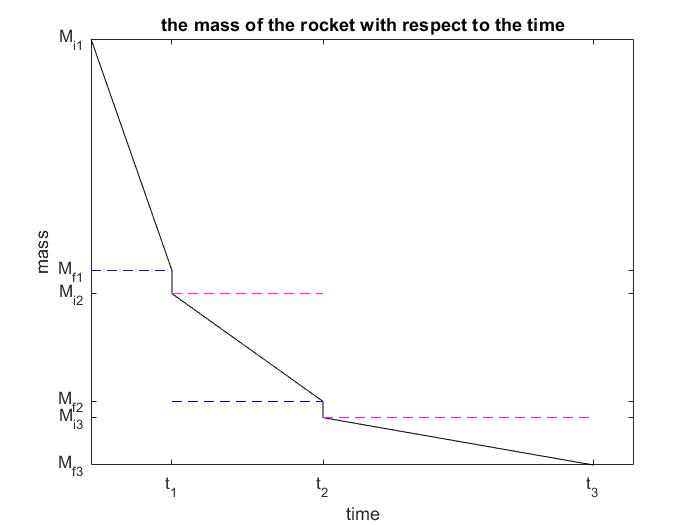
\includegraphics[scale=0.65]{./graphs/mass.jpg}
\caption{masse de la fusée en fonction du temps}
\end{figure}
\end{center}

La masse est bien une fonction affine par morceaux. La masse utile n'a pas été représentée afin de rendre le graphe plus clair.


\end{document}